\def\thefigures{chap4_tomographie/figures}


\section{Introduction}
\label{sec:introduction}

Tomographic inversion schemes aiming at reconstructing the subsurface structures from seismic traveltime data are widely used (e.g. \cite{Rawlinson2010}). The obtained wave propagation velocity distribution is usually a starting point for further analysis at various scales, from near surface to global scale. For a reliable and quantitative interpretation of the tomographic solution, an accurate velocity model with its associated uncertainties are required.

In spite of the fact that the inversion for the velocities is a totally non-linear problem, very often it is solved with iterative linearized approaches that minimize a misfit function. The misfit function usually measures the difference between observed and computed traveltimes as a function of the velocity model parameters. The linearization makes the implicit assumption of a unique solution which is chosen thanks to a regularization procedure that reduces the solution non-uniqueness \citep{Menke2012}. This is generally achieved by imposing the solution to be somehow similar or close to an initial a priori model.

The data-model (traveltimes-velocities) relationship can be highly non-linear and requires the use of global optimization methods. In addition, the linearized approaches are not really adapted to provide reliable uncertainties. From a theoretical point of view, to address these two issues, methods based on Markov Chain Monte Carlo (MCMC) that sample the velocity model parameter space are required, such as reversible-jump MCMC \citep{Green1995, Bodin2009}, Parallel Tempering \citep{Sambridge2014}, or Interactive MCMC \citep{Bottero2016}. These global optimization methods can be applied on non-smooth and non-convex functions as they are derivative-free and produce results independent of the initial model. However, they cannot be parallelized and turn out to be prohibitive in terms of computation time.

Another class of global optimization methods has shown growing interest in the last decades. These methods, known as evolutionary algorithms (EA), are inspired by the natural evolution of species and have demonstrated very good convergence rates. While MCMC methods sample the model parameter space by perturbing iteratively a single model, EA work with a population of simultaneous models that evolve toward better models through stochastic processes. This simultaneous evaluation of independent models implies that it is straightforward to parallelize and thus can significantly reduce the computation time. EA include Genetic Algorithm \citep{Sambridge1992a, Whitley1994}, Differential Evolution \citep{Storn1997, Barros2015}, and Covariance Matrix Adaptation Evolution Strategy \citep{Hansen1996, Grayver2016}.

In this work, we propose to overcome the non-linearity using a rather new EA known as Particle Swarm Optimization (PSO) for its ease of implementation and the low number of tuning parameters required. PSO has been introduced to study birds flocking and fish schooling \citep{Kennedy1995}. While it has been extensively used in other engineering domains (e.g. biomedical, signal processing...) for years, PSO has been fairly ignored by the geophysical community until recently. In seismics, PSO has been applied in history matching for reservoir characterization \citep{Mohamed2010a, FernandezMartinez2012}, traveltime tomography \citep{Tronicke2012, Rumpf2015, Poormirzaee2015}, and surface waves inversion \citep{Wilken2012, Poormirzaee2016}. Yet, PSO may suffer from premature convergence, in particular for functions with complex shapes. Therefore, we propose and describe a simple modification of PSO to tackle premature convergence and improve its robustness. Although PSO is mainly used as a global optimization method, we show that our implementation not only demonstrates better convergence rates, but also samples correctly the model parameter space, allowing more reliable uncertainty quantification. We apply the method on a real 3D microseismic example and sample the model parameter space which allows us to derive reliable velocity model uncertainties.


\section{Theory and method}
\label{sec:theory_and_method}

Geophysical inverse problems are underdetermined optimization problems that can be solved by either linear or non-linear techniques \citep{Tarantola1982}. Let us define the discrete data vector $\mathbf{d} = \left[ d_{1}, \dots, d_{n} \right]^{\top}$, where $n$ is the number of data points. {\color{\revision}Calculated} data are generated by applying the forward modeling operator $g$, most often non-linear, on the model vector $\mathbf{m} = \left[ m_{1}, \dots, m_{p} \right]^{\top}$, with $p$ the number of parameters defining the model

\begin{equation}
	\mathbf{d}^{calc} = g \left( \mathbf{m} \right).
	\label{eq:forward_modeling}
\end{equation}

\noindent Inverse problems consist in determining the model vector $\mathbf{m}$ that minimizes the misfit between the observed data and the {\color{\revision}calculated} data

\begin{equation}
	\mathbf{e} \left( \mathbf{m} \right) = \mathbf{d}^{obs} - \mathbf{d}^{calc} = \mathbf{d}^{obs} - g \left( \mathbf{m} \right).
	\label{eq:error}
\end{equation}

\noindent Given an error vector $\mathbf{e}$ (Equation~\ref{eq:error}), the misfit function is usually defined with an $\ell_{p}$-norm. In geophysical inverse problems, even though other norms can be found in the literature, the $\ell_{2}$-norm is often used

\begin{equation}
	\norm{\mathbf{e} \left( \mathbf{m} \right)}_{2} = \left[ \left( \mathbf{d}^{obs} - g \left( \mathbf{m} \right) \right)^{\top} \left( \mathbf{d}^{obs} - g \left( \mathbf{m} \right) \right) \right]^{\frac{1}{2}}.
	\label{eq:norm2}
\end{equation}

\noindent The non-linearity can be addressed by global optimization methods that explore the model parameter space. In this section, we first describe the PSO algorithm before introducing a more robust implementation based on PSO that tackles its shortcomings.


\subsection{Particle Swarm Optimization}
\label{ssec:particle_swarm_optimization}

For consistency in the notation, the so-called position vector usually denoted by $\mathbf{x}$ in the literature will be denoted by $\mathbf{m}$. Consequently, we will only speak in terms of models instead of position vector.

In PSO, the first step is to generate a swarm composed of several models in the model parameter space. The initial models can either be defined a priori or generated given a random distribution (usually uniform). Each model is represented by a particle that interacts with its neighborhood to find the global minimum of the misfit function. \cite{Kennedy1999} has studied several neighborhood topologies and concluded that the global best topology (all the particles are connected to each other) performed better than the others. Thus, we here only consider the global best topology where the neighborhood of each particle is the entire swarm.

At iteration $k$, a particle~$i$ is defined by a model vector~$\mathbf{m}_{i}^{k}$ and a velocity vector~$\mathbf{v}_{i}^{k}$ and is adjusted according to its own personal best model and the global best model of the whole swarm. The velocity vector controls how a particle moves in the model parameter space and is initialized to zero \citep{Engelbrecht2012}. The velocity and the position of each particle are updated following

\begin{equation}
	\mathbf{v}_{i}^{k} = \omega \mathbf{v}_{i}^{k-1} + \phi_{p} \mathbf{r}_{p}^{k} \left( \mathbf{m}_{p,i} - \mathbf{m}_{i}^{k-1} \right) + \phi_{g} \mathbf{r}_{g}^{k} \left( \mathbf{m}_{g} - \mathbf{m}_{i}^{k-1} \right)
	\label{eq:pso_velocity}
\end{equation}
\begin{equation}
	\mathbf{m}_{i}^{k} = \mathbf{m}_{i}^{k-1} + \mathbf{v}_{i}^{k}
	\label{eq:pso_position}
\end{equation}

\noindent where $\mathbf{m}_{p,i}$ and $\mathbf{m}_{g}$ are respectively the personal best model of particle $i$ and the global best model of the swarm, $\mathbf{r}_{p}^{k}$ and $\mathbf{r}_{g}^{k}$ are uniform random numbers vectors drawn at iteration $k$, $\omega$ is an inertia weight, $\phi_{p}$ and $\phi_{g}$ are two acceleration parameters that respectively control the cognition and social interactions of the particles.

The inertia weight $\omega$ has been introduced by \cite{Shi1998} to help the particles to dynamically adjust their velocities and refine the search near a local minimum. Another formulation using a constriction coefficient based on \cite{Clerc1999} to insure the convergence of the algorithm can be found in the literature. However, \cite{Eberhart2000} showed that the inertia and constriction approaches are equivalent since the parameters are connected.

Empirical studies have concluded that the performance of PSO is sensitive to its control parameters, namely the swarm size $s$, the maximum number of iterations $k_{\max}$, $\omega$, $\phi_{p}$ and $\phi_{g}$. Yet, these studies have provided some insights on the initialization of some parameters \citep{VanDenBergh2006}. \cite{Eberhart2000} empirically found that $\omega = 0.7298$ and $\phi_{p} = \phi_{g} = 1.49618$ are good parameter choices that lead to convergent behaviour. Although these parameters have shown good results in previous studies, be aware that they can also be tuned according to the optimization problem. The sensitivity of PSO to these parameters is analyzed in Section~\ref{ssec:sensitivity_analysis}. Unless explicitly stated, we will set $\omega = 0.7298$ and $\phi_{p} = \phi_{g} = 1.49618$.

The swarm size and the maximum number of iterations have to be carefully chosen dependently of the problem and the computer resources available. These two parameters are related since a smaller swarm will require more iterations to converge, while a bigger swarm will converge more rapidly. In real optimization problems, the computation cost is mainly dominated by the forward modeling. Therefore, the optimization is usually stopped when a predefined number of forward modelings (i.e. computation of misfit functions) is performed. The desired number of forward modelings is controlled by both the swarm size and the maximum number of iterations. \cite{Trelea2003} has studied the effect of the swarm size on several benchmark test functions in 30 dimensions. He found that a medium number of particles ($\approx$~30 particles) gives the best results in terms of number of misfit function evaluations. Too few particles ($\approx$~15 particles) gives a very low success rate while too many particles ($\approx$~60 particles) results in much more misfit function evaluations than needed although it increases the success rate. \cite{Piccand2008} came to the same conclusion with problems of higher dimensions (up to 500).

In the original PSO, the swarm's global best position is updated in a synchronous fashion. In other words, $\mathbf{m}_{g}$ is updated at the end of an iteration once the misfit functions of the entire swarm have been evaluated. \cite{Carlisle2001} has shown that PSO yields better performance when the particles are evaluated asynchronously (i.e. $\mathbf{m}_{g}$ is evaluated after each individual misfit evaluation). Synchronous PSO is intrinsically parallelizable and performs well if the individual misfit function evaluations require the same amount of time, while a parallel asynchronous PSO is not straightforward but could reduce wasted CPU cycles \citep{Schutte2004, Koh2006}. This work only deals with optimization problems with constant misfit computation time, therefore only the synchronous PSO will be considered. The algorithm is described in Algorithm \ref{alg:pso} (\ref{app:algo_pso}).


\subsection{Premature convergence}
\label{ssec:premature_convergence}

The classical implementation of PSO suffers from premature convergence and stagnation as it can be trapped in a local minimum, particularly when the evaluated misfit function has a complex shape. The swarm is said to have stagnated when the particles keep moving in the close vicinity of the global best $\mathbf{m}_{g}$ as particles momentum have faded. We illustrate this statement with the 2D Rastrigin function.

The Rastrigin function is a highly multimodal function commonly used to benchmark global optimization methods due to its complex shape containing several local minima. The function is usually defined in $\left[ -5.12, 5.12 \right]^{n}$ and its global minimum lies in $\left( 0 \right)^{n}$, $n$ being the number of dimensions.

While PSO is able to find the global minimum with $s = 10$~particles, we apply PSO on the 2D Rastrigin function with $s = 5$~particles in order to illustrate the premature convergence (Figure~\ref{fig:pso}). The particles are initialized uniformly in the model parameter space. At iteration~73, PSO has converged prematurely and is trapped in the local minimum $\left( 2, 0 \right)$. At this state, particles inertia have almost vanished and the swarm is stagnating.

\begin{figure}[!htbp]
	\centering
	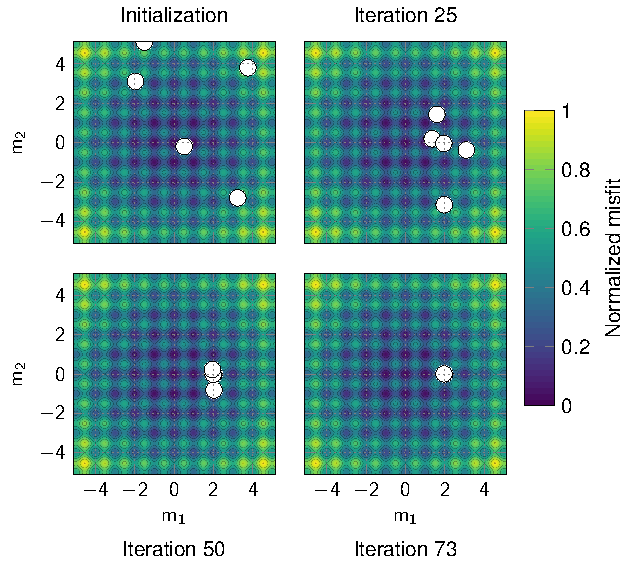
\includegraphics[scale = 1.5]{\thefigures/pso.pdf}
    \caption{Illustration of the premature convergence of PSO on the 2D Rastrigin function with $s = 5$~particles. The 5~particles are uniformly distributed in the model parameter space. Then, the particles converge toward the local minimum $\left( 2, 0 \right)$. From iteration~73, the swarm is trapped in the local minimum.}
    \label{fig:pso}
\end{figure}


\subsection{Competitive Particle Swarm Optimization}
\label{ssec:competitive_particle_swarm_optimization}

To address premature convergence and stagnation state, \cite{VanDenBergh2001} proposed to restart the whole swarm anew. \cite{Evers2009} enhanced the method by adapting the search space at each restart. However, after restarting the whole swarm, the particles may either converge to the same/equivalent or even a worse solution. Therefore, we propose hereby a Competitive PSO (CPSO) to avoid such situations. The idea is to improve the swarm's diversity by renewing part of the population and keeping the ``best'' particles only. ``Worst'' particles are reset, allowing a better exploration of the model parameter space. The newly generated particles will try to look for a better minimum while the ``best'' particles keep searching around the current global best position. If the newest particles find a better minimum, the swarm will gather around the new global best, otherwise they will come back to the current global best until being reset again. We call a reset a ``competition''. Competition is triggered only when premature convergence is detected. \cite{VanDenBergh2001} proposed several methods to detect such state:

\begin{itemize}
	\item Cluster analysis: a percentage of the particles is at a specified Euclidean distance from the global best,
	\item No improvement of the misfit function: the misfit function does not improve significantly over the last iterations,
	\item Swarm maximum radius: the distance of the farthest particle from the global best reaches a certain threshold.
\end{itemize}

\noindent We find that the latter works better in our case. Thus, at the iteration~$k$, competition is triggered if the swarm maximum radius $\delta^{k}$ is smaller than a threshold $\varepsilon$ defined by the user. This condition is written as

\begin{equation}
	\delta^{k} = \max_{1 \le i \le s} \left( \frac{\norm{\mathbf{m}_{i}^{k} - \mathbf{m}_{g}}}{\norm{\mathbf{m}_{\max} - \mathbf{m}_{\min}}} \right) < \varepsilon = \frac{\log \left( 1 + 0.003 s \right)}{\max \left( 0.2, \log \left( 0.01 k_{max} \right) \right)}
	\label{eq:swarm_maximum_radius}
\end{equation}

\noindent where $\norm{\cdot}$ denotes the Euclidean norm. The expression of $\varepsilon$ has been empirically determined and works well for competition triggering since it prevents the swarm from stagnating for too long in a local minimum for any swarm size~$s$. In order to preserve the convergence property of PSO, the proportion of particles to reset should decrease over time. Therefore, we define the proportion of particles to reset at iteration~$k$ by a logistic function $\sigma \left( k \right)$ (Equation~\ref{eq:logistic_function}) parameterized such that it decreases non-linearly with the iteration number. We introduce a competitivity parameter $\gamma \in \left[ 0, 2 \right]$ that controls the position of its inflection point, following

\begin{equation}
	\sigma \left( k \right) = \left( 1 + e^{\frac{1}{0.09} \left( \frac{k}{k_{\max}} - \gamma + 0.5 \right)} \right)^ {-1}
	\label{eq:logistic_function}
\end{equation}

\noindent with $k_{\max}$ the maximum number of iterations. The logistic function is shown in Figure~\ref{fig:logistic} for different values of $\gamma$. The parameters of the logistic function have been empirically tweaked in a way that at early iterations, the swarm is competitive and many particles are reset; at later iterations, we let the swarm stagnate in the last minimum found to refine the solution. $\gamma$ is a problem-dependent parameter. Although we found that $\gamma = 1$ works well in most problems, the parameter can be tuned for faster convergence. A high value of $\gamma$ increases competitivity between particles, resulting in slower convergence. Low competitivity is recommended for unimodal functions (e.g. Spherical function). When $\gamma = 0$ (no competition), CPSO actually behaves like the original PSO since zero particle are reset for any iteration number. The algorithm is presented in Algorithm~\ref{alg:cpso} (\ref{app:algo_cpso}). The competitivity parameter $\gamma$ will be set to 1 from now on.

\begin{figure}[!htbp]
	\centering
	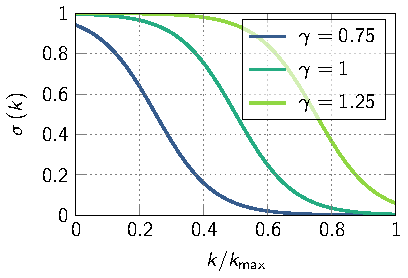
\includegraphics[scale = 1.5]{\thefigures/sigmoid.pdf}
	\caption{Logistic function with different values of competitivity parameter $\gamma$. Increasing $\gamma$ improves the exploration ability (i.e. diversity) of the swarm as more particles are reset. Decreasing $\gamma$ results in faster convergence with higher chance of entrapment in a local minimum.}
	\label{fig:logistic}
\end{figure}

We apply CPSO on the previous example (Figure~\ref{fig:cpso}). Premature convergence is detected at iteration~74 and competition is triggered. A particle finds a better local minimum at iteration~81 which allows the whole swarm to escape from the local minimum and finally gather around the true global minimum. The global minimum is finally found at iteration~186 (the misfit value is lower than a specified threshold). Figure~\ref{fig:gfit} displays the global best misfit value as a function of the iteration number. The black cross marks the iteration when competition has been triggered. The algorithm has required only 1~reset (iteration~74) to be able to find the global minimum.

\begin{figure}[!htbp]
	\centering
	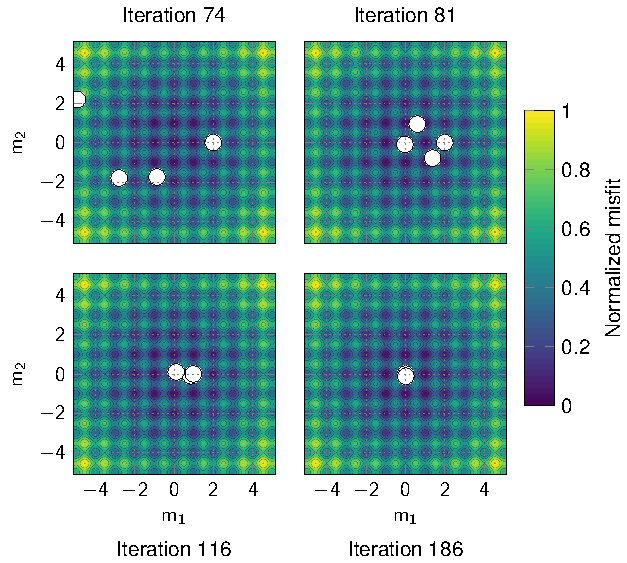
\includegraphics[scale = 1.5]{\thefigures/cpso.pdf}
    \caption{Example of competition triggering. Three~particles are redistributed uniformly in the model parameter space. At iteration~81, one particle has found the central mode which allows the swarm escapes from the previous local minimum. Finally, the swarm has found the global minimum.}
    \label{fig:cpso}
\end{figure}

\begin{figure}[!htbp]
	\centering
	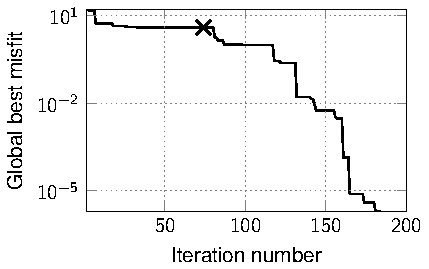
\includegraphics[scale = 1.5]{\thefigures/gfit.pdf}
	\caption{Global best misfit as a function of iteration number. Competition triggering is marked by the black cross (iteration~74). Only one reset has been required for the swarm to escape from a local minimum and eventually find the global minimum.}	
	\label{fig:gfit}
\end{figure}

In this example, CPSO has been able to find the global minimum while PSO fails most of the time with a swarm size of 5~particles. Even though only 1~reset was required for the particles to escape from a local minimum, it should be pointed out that the competition triggering mechanism does not guarantee the swarm to always find a better minimum at each reset, it only improves its chance to escape by improving the swarm's diversity. The next sections are dedicated to the analysis of the robustness of CPSO with respect to its tuning parameters in higher dimensions.


\section{Robustness testing}
\label{sec:robustness_testing}


\subsection{Sensitivity analysis}
\label{ssec:sensitivity_analysis}

We analyze the sensitivity of both PSO and CPSO with respect to the variation of the inertia weight~$\omega$, and the two acceleration parameters~$\phi_{p}$ and $\phi_{g}$ on the Rastrigin function in 5, 10 and 20~dimensions. We vary $\omega$ in the range $\left[ 0, 1 \right]$. In order to facilitate the analysis, we set $\phi_{p} = \phi_{g} = \phi$ and vary $\phi$ in the range $\left[ 0, 3 \right]$. The swarm size is set to 5~times the dimension. For each couple of parameters $\left( \omega, \phi \right)$, 50~trials of 1000~iterations each are performed. The sensitivity with respect to a couple of parameters $\left( \omega, \phi \right)$ is characterized by the success rate (SR) defined as the percentage of trials that yield a misfit lower than a specified threshold. The results of the sensitivity analysis are summarized in Figure~\ref{fig:sensana}.

PSO performs well for a wide range of $\omega$ and $\phi$ with a narrow region of  high SR. This means that $\omega$ has to be chosen dependently of the parameter $\phi$. On the other hand, the high SR region is much wider for CPSO which is therefore more flexible in the choice of $\omega$ and $\phi$. Notice that the control parameters recommended by \cite{Eberhart2000} ($\omega = 0.7298$ and $\phi = 1.49618$) are included in the high SR region. Additional results on the Rosenbrock function are shown in \ref{app:sensitivity_analysis}.

\begin{figure}[!htbp]
	\centering
	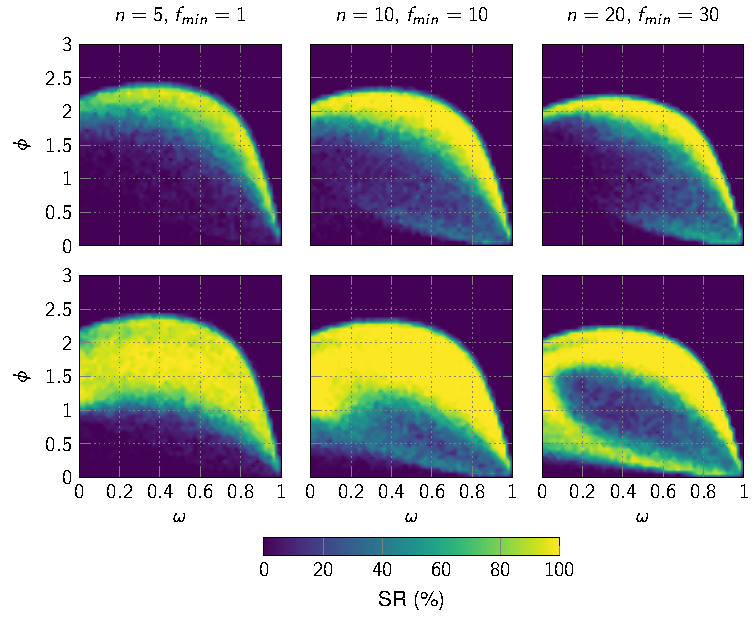
\includegraphics[scale = 1.25]{\thefigures/sensitivity_rastrigin.pdf}
    \caption{Results of the sensitivity analysis to parameters $\omega$ and $\phi$ for PSO (top) and CPSO (bottom) on the Rastrigin function in 5, 10 and 20~dimensions. The swarm size is set to 5~times the dimension and the goal to achieve is indicated by $f_{min}$. CPSO is more flexible in the choice of these parameters as the high SR region is wider than for PSO.}
    \label{fig:sensana}
\end{figure}


\subsection{Benchmark}
\label{ssec:benchmark}

We compare the performances of PSO and CPSO on six classical benchmark test functions (\ref{app:benchmark}) in $n~=~30$~dimensions. Most of the test functions are either unimodal, multimodal or dynamic. Therefore, these benchmark functions are a rather good proxy for assessing the reliability of an optimization method. For both PSO and CPSO, we use $s = 30$~particles and a maximum of $k_{max} = 2000$~iterations. The global minimum misfit is 0 for all the functions tested. The minimum, median and maximum misfit values over 100~independent trials are presented in Table~\ref{tab:benchmark}. We recall that the results have been obtained using synchronized particles.

\begin{table}[!htbp]
	\centering
	\makebox[\textwidth]{
		\begin{tabular}{lccccccc}
			\toprule
			\multirow{2}{*}{Function} & \multicolumn{3}{c}{PSO} & \multicolumn{3}{c}{CPSO} \\
			& Min. & Median & Max. & Min. & Median & Max. \\
			\cmidrule(r){2-7}
			Ackley & 1.377E-13 & 2.814 & 9.539 & 9.766E-13 & 2.092E-10 & 1.502 \\
			Griewank & 0 & 2.951E-02 & 0.244 & 0 & 1.232E-02 & 8.096E-02 \\
			Quartic (noise) & 4.538E-03 & 1.639E-02 & 7.131E-02 & 3.081E-03 & 9.060E-03 & 1.888E-02 \\
			Rastrigin & 32.83 & 68.16 & 135.31 & 12.93 & 28.85 & 50.74 \\
			Rosenbrock & 1.472E-02 & 18.36 & 81.30 & 6.537E-03 & 18.77 & 83.06 \\
			Styblinski-Tang & 56.54 & 141.4 & 226.2 & 1.074E-03 & 56.54 & 113.1 \\
			\bottomrule
		\end{tabular}
	}
	\caption{Results of the benchmark of PSO and CPSO with $s = 30$~particles in $n = 30$~dimensions on six benchmark test functions. The global minimum misfit is 0 for all the functions.}
	\label{tab:benchmark}
\end{table}

\noindent For Quartic (noise) and Rosenbrock (unimodal functions), PSO and CPSO yield similar performance. For the four other functions tested, CPSO has outperformed PSO since the minimum, median and maximum misfit values are lower. While PSO fails to recover the global minimum for the highly multimodal functions Rastrigin and Styblinski-Tang, CPSO shows rather good performances with median misfit much lower compared to PSO. These benchmarks indicate that CPSO is a more robust optimizer than PSO given the same parameters.


\subsection{Importance sampling}
\label{ssec:importance_sampling}

Inversed models obtained through optimization are usually subject to uncertainties introduced by errors in data measurements, in the forward modeling and by the use of a finite number of parameters to describe the model. Therefore, the solution of an optimization problem is not unique as several models can explain the observed data. Uncertainties can be quantified by accounting for all sources of errors in a Bayesian framework and by generating acceptable models that fit the data equally well in terms of misfit function. The posterior Probability Density Function (PDF) is given by the Bayes theorem following

\begin{equation}
	P \left( \mathbf{m} \ \middle| \  \mathbf{d}^{obs} \right) \propto P \left( \mathbf{m} \right) P \left( \mathbf{d}^{obs} \ \middle| \  \mathbf{m} \right)
	\label{eq:bayes_theorem}
\end{equation}

\noindent where the first term $P \left( \mathbf{m} \right)$ is the prior PDF and contains all the information we know about the model $\mathbf{m}$ prior to the measurements of data $\mathbf{d}^{obs}$. The likelihood $P \left( \mathbf{d}^{obs} \ \middle| \  \mathbf{m} \right)$ links the model to the observed data considering that a model that does not explain exactly the data is acceptable to a certain extent, and is written

\begin{equation}
	P \left( \mathbf{d}^{obs} \ \middle| \  \mathbf{m} \right) \propto \exp \left( - E \left( \mathbf{m} \right) \right)
	\label{eq:likelihood}
\end{equation}

\noindent Assuming theoretical normally distributed errors, $E$ is the misfit function and is expressed as

\begin{equation}
	E \left( \mathbf{m} \right) = \frac{1}{2} \left( \mathbf{d}^{obs} - g \left( \mathbf{m} \right) \right)^{\top} \mathbf{\Sigma}^{-1} \left( \mathbf{d}^{obs} - g \left( \mathbf{m} \right) \right)
	\label{eq:ls_misfit}
\end{equation}

\noindent where $\mathbf{\Sigma}$ is the covariance matrix (diagonal for independent observations) that accounts for data measurements and modeling errors \citep{Tarantola2005}.

Ideally, the model parameter space needs to be explored as a whole by estimating $P \left( \mathbf{m} \ \middle| \  \mathbf{d}^{obs} \right)$ for each model $\mathbf{m}$. However, it is not feasible when the number of parameters to estimate is large. Therefore, importance sampling is usually performed through Markov Chain Monte Carlo (MCMC) that generates models distributed according to the PDF when the number of iterations tends toward infinity. We will show how to use CPSO to obtain a rather good approximation of $P \left( \mathbf{m} \ \middle| \  \mathbf{d}^{obs} \right)$.

A single run of PSO does not provide a proper sampling of the model parameter space since it is designed to rapidly locate and exploit a single minimum. \cite{Sen1996} suggests to perform several independent runs of a global optimizer with different starting solutions to sample different parts of the model parameter space. Figure~\ref{fig:pdf} (top) shows 100000~models sampled after 50~runs of 200~iterations of PSO and CPSO on the 2D Rastrigin function. The whole model parameter space is correctly sampled for both PSO and CPSO with particles mainly focused on the central part of the function corresponding to low misfit values (i.e. high probability).

We estimate the distributions for the 100000~previously sampled models by multiple runs of PSO and CPSO with gaussian kernels as shown in Figure~\ref{fig:pdf} (bottom). Even though PSO detects the principal modes, it fails at identifying the central mode as the principal one. For each run, PSO seems to converge prematurely in different local minima without being able to escape from it. On the other hand, CPSO successfully samples the 9~principal modes and the central mode is correctly identified. Therefore, the frequency distribution from multiple runs of CPSO directly provides a rather good approximation of the PDF with no further computation.

\begin{figure}[!htbp]
	\centering
	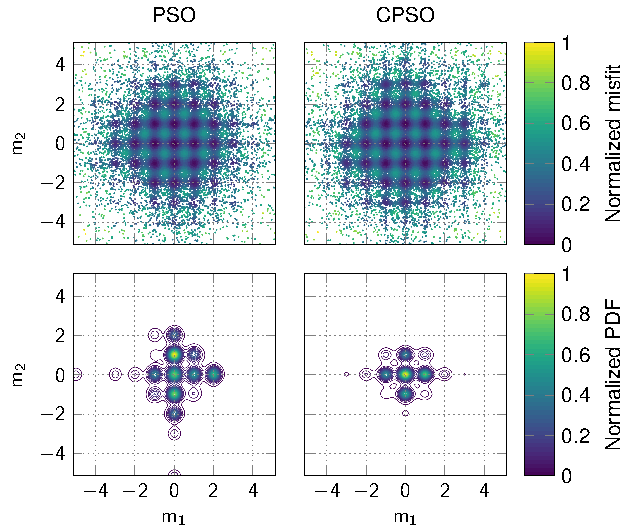
\includegraphics[scale = 1.5]{\thefigures/importance_sampling.pdf}
	\caption{(Top)~100000 models sampled after 50 runs of PSO and CPSO on the 2D Rastrigin function with 5 particles and 200 iterations. The low misfit part of the function is correctly explored by the particles. Similar results can be obtained with more particles. (Bottom)~Frequency distributions of 100000~models sampled by multiple runs of PSO and CPSO on the 2D Rastrigin function. PSO fails at identifying the central mode as the principal one while CPSO correctly identified the 9~central modes.}
    \label{fig:pdf}
\end{figure}

In this section, we have demonstrated the robustness of CPSO as a global optimizer compared to classical implementation of PSO, but also as a more reliable method for uncertainty quantification. We will now apply CPSO on a real first arrival traveltime tomography.


\section{Numerical example}
\label{sec:numerical_example}

In this section, we apply the CPSO tomography algorithm on a real data set recorded in the context of induced seismicity.


\subsection{Acquisition}
\label{ssec:acquisition}

Tomography is a geophysical inverse problem that consists in retrieving the background velocity model from observed first arrival traveltimes of seismic waves recorded at a set of receivers. The geometry used for the acquisition is represented in Figure~\ref{fig:real_data} (left) in a relative Cartesian coordinate system. The monitoring network consists of two wireline arrays of forty 3C-receivers that were deployed in two different vertical wells (white triangles) ranging between 50 and 750~meters depth and regularly spaced every 15~meters. Fifteen perforation shots have been performed along two horizontal wells (green circles) at a depth of 1050~meters. For each of the fifteen perforation shots, almost all 80~first P-wave and approximately 40~S-wave arrivals could be picked. The average P- and S- wave picking uncertainties are estimated to be around 1~ms and 4~ms, respectively.

Acoustic logs for both P- and S-waves have been acquired in one well using a sonic wireline tool. These acoustic logs have been used to derive a layered velocity model consisting of 15~layers (Figure~\ref{fig:real_data} (right)) that will serve as a reference model.

\begin{figure}[!htbp]
	\centering
	\captionsetup[subfigure]{position = top}
	\subfloat{
		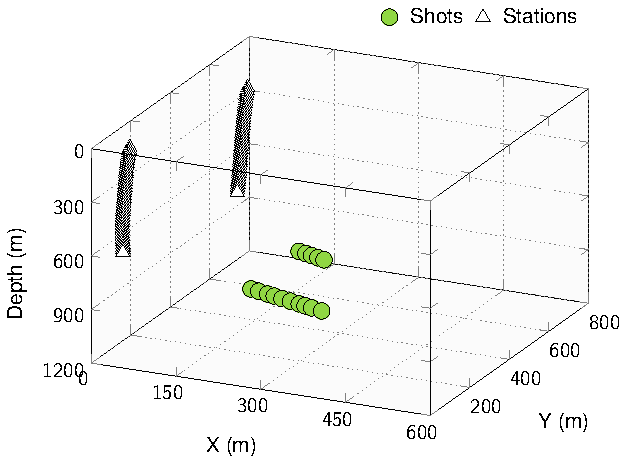
\includegraphics[scale = 0.85]{\thefigures/geometry.pdf}
	}
	\subfloat{
		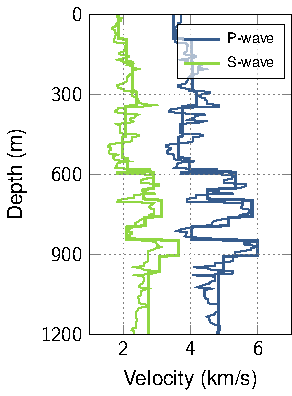
\includegraphics[scale = 1]{\thefigures/velocity_profiles.pdf}
	}
	\caption{(Left)~3D acquisition geometry with perforation shot locations (green circles) and receiver locations (white triangles). (Right)~Acoustic logs and 1-D reference calibrated velocity models for P-wave (blue) and S-wave (green).}
	\label{fig:real_data}
\end{figure}

The acquisition geometry is poorly constrained and requires the solution to be represented in terms of PDF through a Bayesian formulation. We also expect to obtain greater uncertainties for the S-wave velocity model since we have fewer arrival times associated to S-waves. 


\subsection{Inversion results}
\label{ssec:inversion_results}

The velocity model is parameterized with 15~layers based on the reference model, and we invert for the P-wave velocity $V_{p}$, the ratio $V_{p}/V_{s}$ and the interface depth of each layer. Therefore, the model consists of 45~unknown parameters. The lower and upper boundaries of each layer parameters are summarized in Table~\ref{tab:search_space}.

\begin{table}[!htbp]
	\centering
	\makebox[\textwidth]{
		\begin{tabular}{ccccccc}
			\toprule
			\multirow{2}{*}{Layer \#} & \multicolumn{2}{c}{$V_{p}$ (m/s)} & \multicolumn{2}{c}{$V_{p}/V{s}$} & \multicolumn{2}{c}{Depth (m)} \\
			& Min. & Max. & Min. & Max. & Min & Max. \\
			\cmidrule(r){2-7}
			1 & 2500 & 5000 & 1.5 & 2.2 & 90 & 110 \\
			2 & 2500 & 5000 & 1.5 & 2.2 & 172 & 192 \\
			3 & 2500 & 5000 & 1.5 & 2.2 & 273 & 305 \\
			4 & 3000 & 5500 & 1.5 & 2.2 & 340 & 360 \\
			5 & 2500 & 5000 & 1.5 & 2.2 & 450 & 480 \\
			6 & 2500 & 5000 & 1.5 & 2.2 & 530 & 550 \\
			7 & 2500 & 5000 & 1.5 & 2.2 & 580 & 600 \\
			8 & 3500 & 6500 & 1.5 & 2.2 & 650 & 670 \\
			9 & 3000 & 6000 & 1.5 & 2.2 & 690 & 710 \\
			10 & 4000 & 7000 & 1.5 & 2.2 & 750 & 775 \\
			11 & 3500 & 6500 & 1.5 & 2.2 & 790 & 810 \\
			12 & 3000 & 6000 & 1.5 & 2.2 & 840 & 860 \\
			13 & 3500 & 7000 & 1.5 & 2.2 & 900 & 920 \\
			14 & 3500 & 6500 & 1.5 & 2.2 & 960 & 980 \\
			15 & 3000 & 6500 & 1.5 & 2.2 & 1200 & 1200 \\
			\bottomrule
		\end{tabular}
	}
	\caption{Lower and upper boundaries of each layer parameters. Particles are uniformly initialized in the search space.}
	\label{tab:search_space}
\end{table}

Traveltimes are calculated using an eikonal solver that generates traveltime grids for each perforation shots \citep{Noble2014}. We run the CPSO algorithm 50~times to sample the model parameter space sufficiently for uncertainty quantification with different swarm sizes (16, 32, 64 and 128~particles). A run is stopped when 200~iterations are performed. The four tomographies lasted respectively 1.8~minutes, 3.6~minutes, 7.2~minutes and 14.3~minutes using a total of 96~cores {\color{\revision}out of 104 (four sockets platform made of 4~Intel$^{\mbox{\scriptsize{\textregistered}}}$ Xeon$^{\mbox{\scriptsize{\textregistered}}}$ Platinum 8164 CPU, 26~cores @ 2.00~GHz each)}. To allow comparison with MCMC, we also run a Monte Carlo tomography that consists of 1~million models sampled using the Metropolis-Hastings algorithm which lasted 1.3~hours using 15~cores for the parallelization of the forward problem.

Figure~\ref{fig:fitness} represents the evolution of the misfit with respect to the iteration number for Monte Carlo tomography (left) and the four CPSO tomographies (right). It shows that despite the 45~parameters to invert, a swarm size of $s = 16$ was actually enough to recover a good velocity model. We can also notice that increasing the swarm size allows the swarm to converge faster which was expected. Besides, Monte Carlo tomography required more than 10000~iterations to reach its stationary regime, while CPSO tomographies needed less than 100~iterations (i.e. less than 1600~concurrent misfit function evaluations in the best case) to converge. In terms of optimization performance, this means a gain of 2~orders of magnitude compared to MCMC.

\begin{figure}[!htbp]
	\centering
	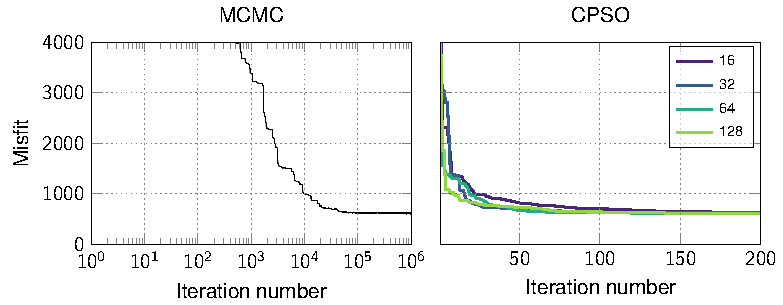
\includegraphics[scale = 1.25]{\thefigures/fitness.pdf}
	\caption{(Left)~Energy (or misfit) of the Markov Chain as a function of the iteration number. The algorithm required more than 10000~iterations to reach equilibrium. (Right)~Global best misfits for the best models with respect to the iteration number for different swarm sizes. In the four cases, the misfit function values are equivalent at the last iteration.}
	\label{fig:fitness}
\end{figure}

The best and mean models are respectively represented in green and blue in Figure~\ref{fig:velocity_models}. The mean model is calculated as the weighted sum of all the models sampled and is written as

\begin{equation}
	\hat{\mathbf{v}} = \frac{\sum_{i = 1}^{s \times k_{max}} P \left( \mathbf{m_{i}} \ \middle| \  \mathbf{d}^{obs} \right) \mathbf{v_{i}}}{\sum_{i = 1}^{s \times k_{max}} P \left( \mathbf{m_{i}} \ \middle| \  \mathbf{d}^{obs} \right)}
	\label{eq:mean_model}
\end{equation}

\noindent where $\mathbf{v_{i}}$ is the continuous velocity model transformed from the parameters $\mathbf{m_{i}}$. The velocity models obtained from the different tomographies are remarkably similar and seem consistent with the acoustic logs for both P- and S-waves.

\begin{figure}[!htbp]
	\centering
	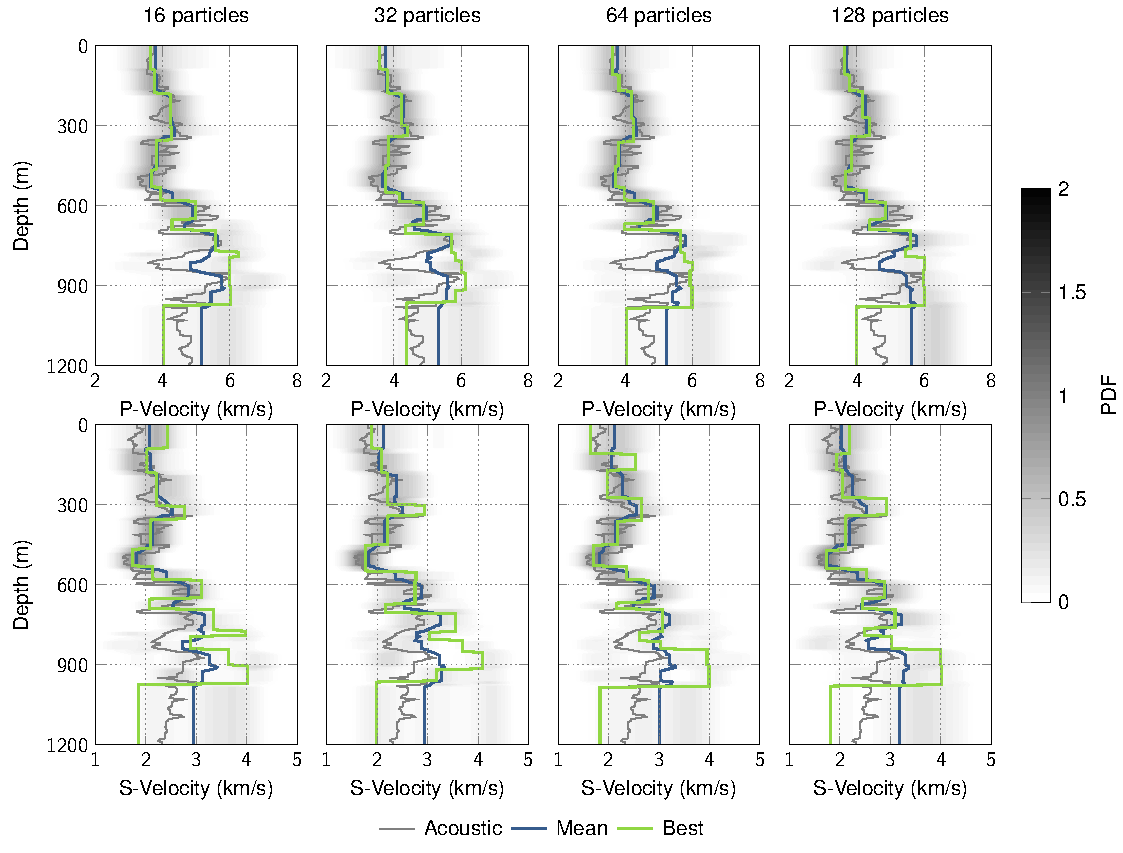
\includegraphics[scale = 0.8]{\thefigures/velocity_models.pdf}
	\caption{P- and S-waves velocity models obtained with 16~particles, 32~particles, 64~particles and 128~particles. The acoustic logs are represented in black, the best velocity models in green, the mean velocity models in blue, and the density plots in gray scale, darker colors indicating higher probabilities. Results are remarkably similar in the four cases.}
	\label{fig:velocity_models}
\end{figure}

The velocity uncertainties are represented by the density plots, darker colors indicating higher probabilities. We display in Figure~\ref{fig:uncertainties} the marginal probabilities at three different depths (300, 600 and 900~meters). The marginal probabilities are narrow at 300 and 600~meters depth which correspond to the constrained region where the receivers are deployed, and is almost uniform at 900~meters depth (below the receivers). Also, the marginal probabilities obtained for the S-wave velocity models are thicker than those of P-wave velocity models as we have fewer arrival time picks associated to S-waves. These marginal probabilities are consistent with the acquisition geometry and the ray coverage between the sources and the receivers and are in agreement with the ones obtained with a MCMC sampler. Besides, the velocity uncertainties obtained for the four tomographies do not differ much from each other, which means that uncertainty quantification in first arrival traveltime tomography using CPSO is relatively insensitive to the swarm size.

\begin{figure}[!htbp]
	\centering
	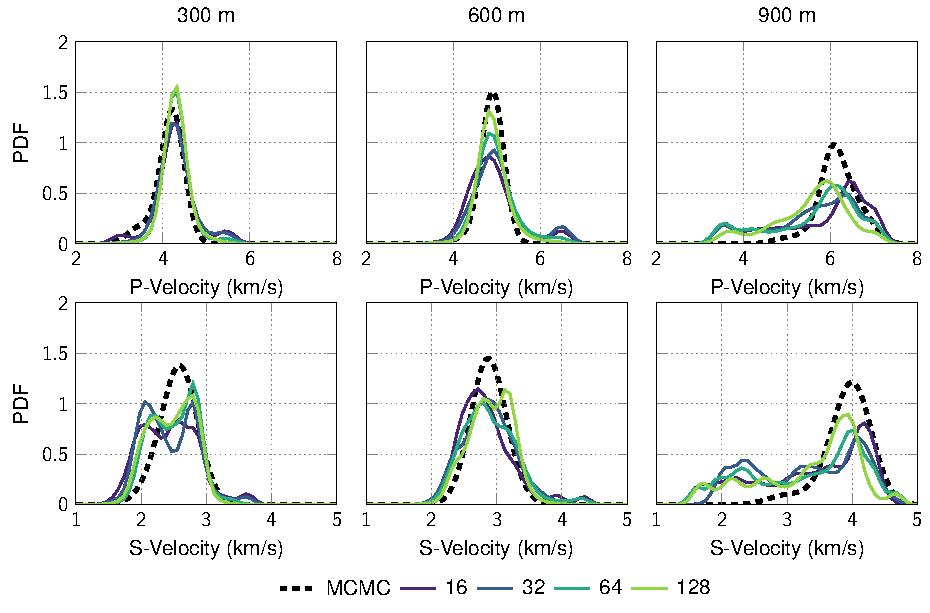
\includegraphics[scale = 1]{\thefigures/uncertainties.pdf}
	\caption{Marginal probabilities at 300, 600, and 900~meters depth obtained with different swarm sizes (16, 32, 64, 128~particles) and MCMC. Probabilities are narrow at 300 and 600~meters depth where the receivers are deployed, and wide at 900~meters below the receivers. Marginal probabilities obtained with CPSO are in agreement with the ones obtained with MCMC.}
	\label{fig:uncertainties}
\end{figure}

Finally, we relocate the fifteen perforation shots using an hybrid approach in the four best velocity models obtained with different swarm sizes, and in the calibrated reference velocity model as well. First, we perform a grid search over the hypocenter parameter space. Then, we refine the search around the solution found by the grid search using CPSO. Figure~\ref{fig:locations_diff} represents the location errors for each perforation shots in the X, Y and Z~directions. In the reference model, we observe a mean absolute location error of 10, 7 and 12~meters in the X, Y and Z~directions, respectively. In our four velocity models, the fifteen shots are accurately relocated in the Y and Z~directions with a mean absolute error of 2 and 3~meters. Yet, the mean absolute location error in the X~direction is about 10~meters. This may be due to the poor ray coverage in this direction and by the fact that we did not take into account a potential anisotropy in the medium.

\begin{figure}[!htbp]
	\centering
	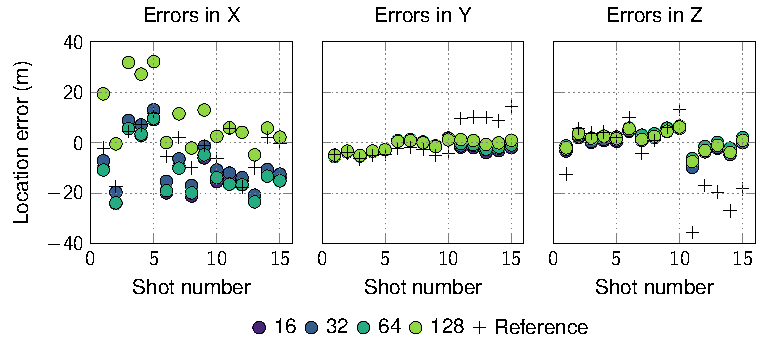
\includegraphics[scale = 1.25]{\thefigures/locations_diff.pdf}
	\caption{Location errors in X, Y and Z directions for the four best velocity models obtained with different swarm sizes (16, 32, 64, 128~particles). The black crosses represent the location errors in the reference model. The shots are accurately relocated in the Y and Z~directions but the mean absolute location error in the X~direction is about 10~meters.}
	\label{fig:locations_diff}
\end{figure}

All in all, the locations obtained from our four velocity models are more accurate, especially in depth, which indicates that velocity models obtained from CPSO tomography can be reliably used in microseismic monitoring. 


\section{Hybrid parallel implementation}
\label{sec:hybrid}

In the last decades, High Performance Computing (HPC) has gain growing interest in geophysics as it provides an integrated solution to solve large scientific and engineering problems. Today's supercomputers are systems made of Symmetric Multi-Processors machines (SMP) and therefore combine features of shared and distributed memory architecture \citep{Rabenseifner2009, Drosinos2004}. This allows multi-levels hybrid parallel programming where message passing model (MPI) is employed between processes (or ranks), and shared memory model (OpenMP) is used for each process.

Non-linear traveltime tomography is a heavy computational problem that requires a lot of forward modeling (i.e. computation of traveltimes). In our microseismic example, a traveltime grid is computed for each perforation shot. Each grid can be computed independently which allows a first level of parallelism. Besides, unlike MCMC methods usually applied in geophysical problems, EA such as PSO have the advantage to evaluate concurrently a population of models, which add another level of parallelism. In our hybrid parallel implementation, we evenly distribute the particles to the MPI processes. Therefore, our implementation requires the swarm size to be a multiple of the number of available {\color{\revision}cores} for maximum efficiency to avoid idle {\color{\revision}cores}. For each process, given a velocity model defined by the particle, the computation of the traveltime grids for each perforation shots are scattered over the threads with OpenMP.

We evaluate the parallel performance of our implementation on our real tomography example by calculating the speed up and parallel efficiency for different number of {\color{\revision}cores}. The speed up is defined as the ratio of sequential computation time to parallel computation time. Parallel efficiency is the ratio of speed up to the number of {\color{\revision}cores}. Ideally, speed up and parallel efficiency should equal the number of {\color{\revision}cores} and 1, respectively. We solve our tomography problem with 104~particles and 100~iterations on {\color{\revision}the 104~cores of a 4~sockets SMP machine (each processor having 26~cores)}, and perform 5~runs using 1, 13, 26, 52 and {\color{\revision}104~cores with only 1~OpenMP thread, which corresponds to a strong scaling analysis}. Results of parallel performance are reported in Figure~\ref{fig:scalability}.

\begin{figure}[!htbp]
	\centering
	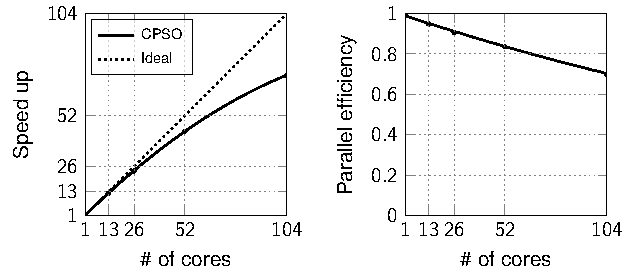
\includegraphics[scale = 1.25]{\thefigures/scalability.pdf}
	\caption{Parallel performance of CPSO on a real tomography problem. (Left)~Speed up. (Right)~Parallel efficiency.}
	\label{fig:scalability}
\end{figure}

Overall, increasing the number of {\color{\revision}cores} reduces the computation time. However, speed up is not ideal {\color{\revision}(72 at 104~cores)} and parallel efficiency decreases almost linearly with increasing number of {\color{\revision}cores}. Therefore, the algorithm becomes less efficient by adding more and more {\color{\revision}cores}. This is due to communication overhead and/or overhead implied by parallel decomposition of the algorithm. An asynchronous parallel implementation could improve PSO scalability and allow close to ideal parallel performance \citep{Koh2006, Venter2006, Mussi2011}.


\section{Discussion and conclusion}
\label{sec:discussion_and_conclusion}

With the rise in computational power that we have witnessed in the recent years~--~in particular with the emergence of multi-cores machines~--~it is important to implement algorithms that are able to handle efficiently all the available CPU resources. EA such as PSO are global optimization methods that evaluate simultaneously a set of independent solutions, implying a straightforward parallelization of these algorithms.

In this paper, we have introduced a new algorithm based on PSO for non-linear first arrival traveltime tomography that we called CPSO. We have demonstrated its robustness in finding a good fitting solution on several benchmark test functions, and even in appraising reliably uncertainties when run multiple times. CPSO has been successfully applied on a real 3D~microseismic example in the context of induced seismicity with reliable uncertainties indicating which parts of the velocity models are well constrained. The velocity models sampled by multiple runs of CPSO can be used to propagate velocity uncertainties to microseismic event locations. Indeed, \cite{Gesret2015} showed that more accurate locations with more reliable uncertainties can be obtained by taking into account both traveltime picking and velocity errors.

We have shown that CPSO is less sensitive to its main tuning parameters in addition to the swarm size. Unfortunately, there is no rule-of-thumb for this parameter as the swarm size is highly dependent on the problem (i.e. the dimension, the landscape). In our tomography example, we have shown that 16~particles are enough in spite of the number of unknowns to invert (45~parameters). Increasing the swarm size improves the speed of convergence as it enhances the exploration capability of the swarm, yet it does not improve much the final model.

In our implementation, we have parallelized the computation of the forward problem at two levels: the individuals are evaluated simultaneously among different MPI processes, and the traveltime grids of each perforation shot are calculated concurrently by different OpenMP threads. Another approach of parallelization are the island models where the EA are parallelized themselves \citep{Gong2011, Gong2015}. In other words, the initial population is divided into subpopulations that evolve independently on a subset of {\color{\revision}cores} (the islands) with a periodical exchange of individuals (migration). It has been shown that island model EA yield better performance as each population follows a different evolution path \citep{Whitley1999}. The migration process is analogous to the exchange of states in Parallel Tempering and Interactive MCMC. One can also consider that each subpopulation evolves following different stochastic processes, which has led to hybrid island model based evolutionary algorithms. The advantage of these algorithms is that by combining different EA, the shortcomings of one can be compensated by another.

In our tomography algorithm, we assumed that the picking errors were known. In practice, observation picking uncertainties are usually poorly determined. \cite{Malinverno2004} addressed this issue with a Hierarchical Bayesian formulation that assigns the measurement errors as unknowns of the inverse problem, which allows the algorithm to infer the level of noise that fit the data the best. Our algorithm can be extended to such formulation with very little modification.

CPSO can also be applied on other geophysical inversion problems that require a global optimization method (e.g. earthquake location, estimation of focal mechanism, inversion of dispersion curves). The competitivity concept introduced in this paper can, as well, be adapted to other EA that suffer from premature convergence such as Differential Evolution.